\documentclass{life-fr}
\usepackage{eurosans}
\usepackage{totpages}

\begin{document}

\title{La Vie est un Jeu}
\subtitle{Cahier des charges}
\member{Lepage Barbara}{lepage.barbara@gmail.com}
\member{Caradec Guillaume}{guillaume.caradec@gmail.com }
\member{Corsin Simon}{simoncorsin@gmail.com }
\member{Glorieux François}{fra.glorieux@gmail.com}
\member{Klarman Nicolas}{nickoas@gmail.com}
\member{Lassagne David}{david.lassagne@gmail.com}
\member{Louvigny Guillaume}{guillaume@louvigny.fr}
\member{El-Outmani Youssef}{youssef.eloutmani@gmail.com}
\member{Le-Cor Wilfried}{wilfried.lecor@gmail.com}
\member{Lenormand Frank}{lenormf@gmail.com}

\summary
{
  Le cahier des charges vise à définir les « spécifications de base »
  de notre service.
}

\maketitle
\authorspage

%% --------------------------------------------------------------------- %%

\chapter*{Résumé}
{
  ``La Vie Est Un Jeu'' est un projet sur 3 ans dans le cadre des ``Epitech
  Innovative Projects'' grâce à un groupe de 10 étudiants.\\
  \\
  Ce projet, sous forme d'un site web et d'applications mobiles, propose à
  ses utilisateurs de pimenter leurs quotidiens. Pour cela, on leur propose
  de manière ludique de se fixer des objectifs, les réaliser, les collectionner
  et enfin les partager.\\
  C'est donc à la fois un jeu et un réseau social, destiné à tout les âges !\\
  \\
  Le site web proposera comme première vue des diapositives de présentation du
  projet. La page d'accueil de l'utilisateur une fois connecté contiendra un
  flux d'informations courtes (par exemple quand un utilisateur s'est fixé un
  objectif) ou longues : quand un utilisateur a réalisé un objectif et le partage.
  \\\\
  La page profil de l'utilisateur contiendra un tableau de médailles représentant
  les objectifs qu'il a réalisé. On appelle les objectifs réalisés des
  ``achievements'', en rapport avec ceux que l'on peut trouver dans les jeux
  vidéos.\\
  \\
  Le projet sera réalisé en utilisant une technologie récente et innovante :
  Ocsigen, un puissant serveur web et framework en OCaml.\\
  Le serveur web sera hebergé sur une Dedibox.\\
  \\
  L'équipe se travaillera de manière judicieuse afin de mener à bien le projet
  malgré la distance séparant les membres. En effet, pendant toute la deuxième
  année de réalisation du projet, les membres seront tous dispersés à travers
  le monde pour une année universitaire obligatoire à l'étranger.\\
  \\
  Ce projet est ambitieux par son pari technique, avec l'utilisation d'une
  technologie peu connue, mais aussi par son succès recherché auprès de ses
  futurs utilsateurs.
}

\chapter*{Informations du document}

\begin{tabular}{ | m{5cm} | m{10cm} | }
  \hline
  Type du document & Cahier des Charges\\
  \hline
  Nom du groupe & La Vie Est Un Jeu\\
  \hline
  Nombre de pages & \ref{TotPages} \\
  \hline
  Titre complet du document & Cahier des Charges du projet ``La Vie Est Un Jeu''\\
  \hline
  Auteurs & Membres du groupe, voir page de garde\\
  \hline
  Responsable & Chef de groupe : Barbara Lepage\\
  \hline
  Contact & lavieestunjeu@googlegroups.com\\
  \hline
  Mots clés & ``cahier des charges'', ``lavieestunjeu''\\
  \hline
  Révision actuelle & 2.1\\
  \hline
  Site vitrine & http://eip.epitech.eu/2014/lavieestunjeu/\\
  \hline
  Site officiel & Non disponible\\
  \hline
\end{tabular}

\chapter*{Table des révisions}

\revision{1.0}{Lepage Barbara}{Rappel de l'EIP}{05/04/2012}
\revision{1.1}{Louvigny Guillaume}{Principe de base du système futur}{05/04/2012}
\revision{1.2}{Lepage Barbara}{Environnement matériel}{05/04/2012}
\revision{1.3}{Lenormand Frank}{Environnement de réalisation}{05/04/2012}
\revision{1.4}{Lenormand Frank}{Architecture technique}{05/04/2012}
\revision{1.5}{Klarman Nicolas}{Gestion de la sécurité}{05/04/2012}
\revision{1.6}{Lepage Barbara}{Points sensibles}{05/04/2012}
\revision{1.7}{Le-Cor Wilfried}{Description des tests de premier niveau}{05/04/2012}
\revision{1.8}{Lassagne David}{Schéma de la base de données}{05/04/2012}
\revision{2.0}{Lepage Barbara}{Mise à jour du résumé et remaniement du plan global}{01/07/2012}
\revision{2.1}{Guillaume Louvigny}{Reprise de la partie applications mobiles et corrections mineures}{05/07/2012}
\listofrevisions

\newpage

\tableofcontents


%% --------------------------------------------------------------------- %%

\chapter{Introduction}

Le présent cahier des charges est un document contractuel visant à définir les
spécification de ``La Vie est un Jeu'', notre EIP.\\
Il précise l’ensemble des fonctionnalités, en plus de l’architecture du site et
des applications mobiles.\\
La structure interne de la base de données sera également décrite.\\
Ce document détaillera également les cibles potentielles du projet et tentera
d’estimer les contraintes financière et temporelles nécessaire pour mener à bien
la réalisation de ce projet.\\
Enfin, l’ouverture offerte aux programmeurs tiers sera également abordée.


%% --------------------------------------------------------------------- %%

\chapter{Epitech, l'EIP et ``La Vie Est Un Jeu''}

\section{Epitech, une école d'informatique pas comme les autres}

Epitech est une école formant des experts en informatique. Sa pédagogie par projets
implique directement les étudiants dans leur apprentissage et les rend plus à même
de réagir et s'adapter aisément, par exemple aux évolutions technologiques qui
auront lieu au cours de leur carrière.

\section{L'EIP, élément clé de la réussite scolaire}

Un Epitech Innovative Project ou EIP est l'élément clé du cursus Epitech. Il s'agit d'un projet de fin d'études regroupant un minimum de six étudiants autour d'un but commun. Ce projet est conduit sur une durée de trois ans, beaucoup plus importante que celles des projets réalisés lors des trois premières années d'études. De plus, l'EIP amène les étudiants à se confronter au monde de l'entreprise.

\section{« La vie est un Jeu », bien plus qu'un simple EIP : une révolution !}

Dans le cadre de notre EIP, nous avons décidé de réaliser un réseau social à but ludique basé sur les « listes de choses à faire avant de mourir » : elle définit toutes les choses que son auteur désire faire de son existence, une sorte de mémo pour ne pas gâcher sa vie. Notre projet permettra à nos visiteurs de construire leurs propres listes et de faire valider leurs exploits tout en les partageant avec leurs réseaux sociaux. Ainsi, chaque action réalisée par un utilisateur (ajout d'une activité, succès ou échec) sera un fil de discussion dans lequel le visiteur et son réseau pourra discuter et partager différents types de médias (photos, vidéos, etc.). Ce fil de discussion se trouvera sur les flux d'informations propres à chacun. L'activité d'un utilisateur sera validée par son propre réseau et apparaîtra sous forme de « succès », comme dans un jeu vidéo. Le site s'étendra par la suite en proposant d'autres caractéristiques propres aux jeux vidéo.

%% --------------------------------------------------------------------- %%

\chapter{Pré-requis et informations sur le projet}

\section{Destinataires du projet}

Les utilisateurs ciblés par le projet sont très nombreux. Il suffit qu'une personne ait un centre d'intérêt ou une passion couvert(e) par le site pour qu'elle ait une raison de s'y inscrire.\\

Le site comme les applications mobiles seront conçus en vue d'une internationalisation étendue.

\section{Utilisation du projet, rapport à l'existant}

Pour les utilisateurs finaux, le projet sera composé d'un site web et de plusieurs applications mobiles incluant Android, iOS et Windows Phone. Pour les développeurs tiers, une API sera créée permettant la création de nouveaux usages.\\

Le projet est créé pour pouvoir répondre à un ensemble de fonctionnalités non présentes dans les projets déjà existants. Ces fonctionnalités ne sont pas combinées ou présentes sur les sites concurrents. En effet, nous tenons à mettre en place une plateforme suffisamment ludique pour être visitée au quotidien, sans pour autant négliger l’aspect social permettant au visiteur de discuter de ses loisirs avec son réseau et de pouvoir partager aisément ses expériences à travers photos et vidéos.\\

À l'issue de la première année de travail sur le projet en partenariat avec l'INRIA et le Koalab Epitech, nous estimons avoir un site fonctionnel. Pendant la seconde année de travail sur l'EIP nous aimerions pouvoir signer des partenariats commerciaux avec divers acteurs de domaines culturels ou encore événementiels. Cette période sera également l'occasion d'ajouter de nouvelles fonctionnalités annexes répondant à des besoins émanant par exemple des utilisateurs.

\newpage

\section{Remise en contexte technologique}

Aujourd'hui, une part de plus en plus importante des utilisateurs d'Internet sont équipés en smartphones, il est même prévu que le nombre d'utilisateurs en mobilité dépasse celui des utilisateurs sédentaires d'ici quelques années.\\
\\
Pour s’adapter à cette évolution et faire face à l’expansion notable de nouvelles technologies, nous avons choisi de proposer à nos utilisateurs des versions dédiées aux plateformes mobiles majeures.

\section{Qu'est-ce qu'un ``Achievement'' ?}
Le terme achievement (qui peut être traduit par succès ou réalisation en français) est, dans le cadre vidéoludique,  un objectif défini à accomplir par le joueur, en dehors de l’objectif principal (c’est-à-dire, gagner ou finir le jeu).\\
 Les achievements sont donc des récompenses honorifiques ajoutant du challenge pour le joueur.\\
\\
Nous pourrions utiliser une traduction française du terme achievement mais nous pensons que achievement est le terme le plus populaire dans le monde vidéoludique.\\
\\
Les achievements permettent au joueur de découvrir plus en profondeur le contenu du jeu et donc d’explorer de nouveaux horizons.\\
 L’obtention est souvent un moment agréable pour le joueur.\\
 Il ressent une certaine satisfaction et se sent récompensé pour un effort.\\
 Il peut ensuite les partager avec ses amis afin de recueillir les honneurs ou de défier ses amis de faire autant ou mieux, ce qui améliore grandement l’immersion au sein du jeu.\\
\\
Nous pensons, qu’il est intéressant d’en faire une analogie avec la vie.\\
 La vie est un jeu comme un autre et mérite d’avoir elle aussi ses achievements.

\section{But final du projet}

Le projet a pour but de créer une communauté d'utilisateurs autour d'un système d'« achievements », directement lié à la vie quotidienne, aux passions ou à la vie professionnelle.\\

Les utilisateurs ciblés sont très nombreux. En théorie, toute personne ayant un centre d'interêt ou une passion est une cible.\\

À plus long terme, des partenariats commerciaux permettront de cibler des marques et des lieux.\\

Le site sera multilingue, donc ouvert à l'internationalisation.

%% --------------------------------------------------------------------- %%

\chapter{Description des différentes parties des services internet et mobiles}

\section{Le Site Web}

\subsection{Vue d'ensemble de la page d'accueil avant le login}

L'utilisateur verra en premier lieu un diaporama mettant en avant certains « achievements », classés par date de publication et par popularité, ainsi que les diverses fonctions du site. Ce diaporama aura pour but d'inciter à l'utilisateur à procéder à son inscription.\\

La page d'accueil permettra également à l'utilisateur de s'inscrire au site. Cette inscription est détaillée plus loin.\\

La dernière fonctionnalité principale de cette page d'accueil est la connexion de l'utilisateur au site.\\

L'entrée du site pourrait éventuellement permettre de rechercher les « achievements » et catégories de celui-ci.

\newpage

\subsection{L'inscription, les cinq premières minutes !}

L'objectif de cette étape serait clairement d'éviter toute la lourdeur que représente la récolte d'informations que le site a besoin d'effectuer auprès du futur utilisateur (présenter un formulaire compact et sauvage a des chances de rebuter celui-ci et éventuellement de le faire renoncer à son inscription).\\

Nous avons donc pensé à un système en mode pas à pas qui, tout en faisant découvrir notre outil et son univers à l'internaute, lui ferait de subtiles demandes d'informations de façon régulière, et ce afin d'alléger cette étape essentielle qui nous permettra de catégoriser le nouvel inscrit et de lui proposer du contenu en fonction de ces informations qui auront été récoltées.\\

En plus de combiner le rôle de « guide » pour la découverte du site et de « sondeur » pour la récolte d'informations, cette méthode a pour avantage de pousser l'utilisateur à aller au bout de la présentation, et donc de l'inscription, au fur et à mesure de son avancée (effet psychologique, il veut finir ce qu'il a commencé, puisqu'il a déjà commencé à contribuer, autant aller jusqu'au bout). La présentation allant, l'intérêt croissant, les chances d'une inscription augmentent à l'arrivée.\\
\\

Dans l'état actuel on imagine comme première approche une question simple qui amène à faire une simple action en mode « vous êtes à un clic de rentrer dans notre univers » avec, par exemple, le choix du genre : Homme, Femme, Non précisé.

\begin{figure}[H]
  \begin{center}
    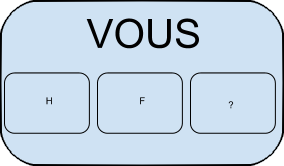
\includegraphics[width=10cm]{img/vous.png}
  \end{center}
\end{figure}

\newpage

\subsection{La page d'accueil utilisateur une fois connecté}

La page d'accueil de l'utilisateur habitué au site présente son flux d'informations, à l'image des flux habituels de sites communautaires tels que Facebook ou Google+. \\

Le menu doit être discret. L'utilisateur doit tout de suite voir les quatre onglets principaux :

\begin{itemize}
  \item le flux (page d'accueil par défaut) ;
  \item les objectifs de l'utilisateur (ses inscriptions) ;
  \item les « achievements » ;
  \item les « amis » de l'utilisateur (importés des réseaux sociaux ou ajoutables dans le cadre du site).
\end{itemize}

Une barre de « breaking news » en permanence en haut du site donnera à l'utilisateur en une ligne les derniers « achievements » de ses amis ainsi que les nouveautés du site.

\begin{figure}[H]
  \begin{center}
    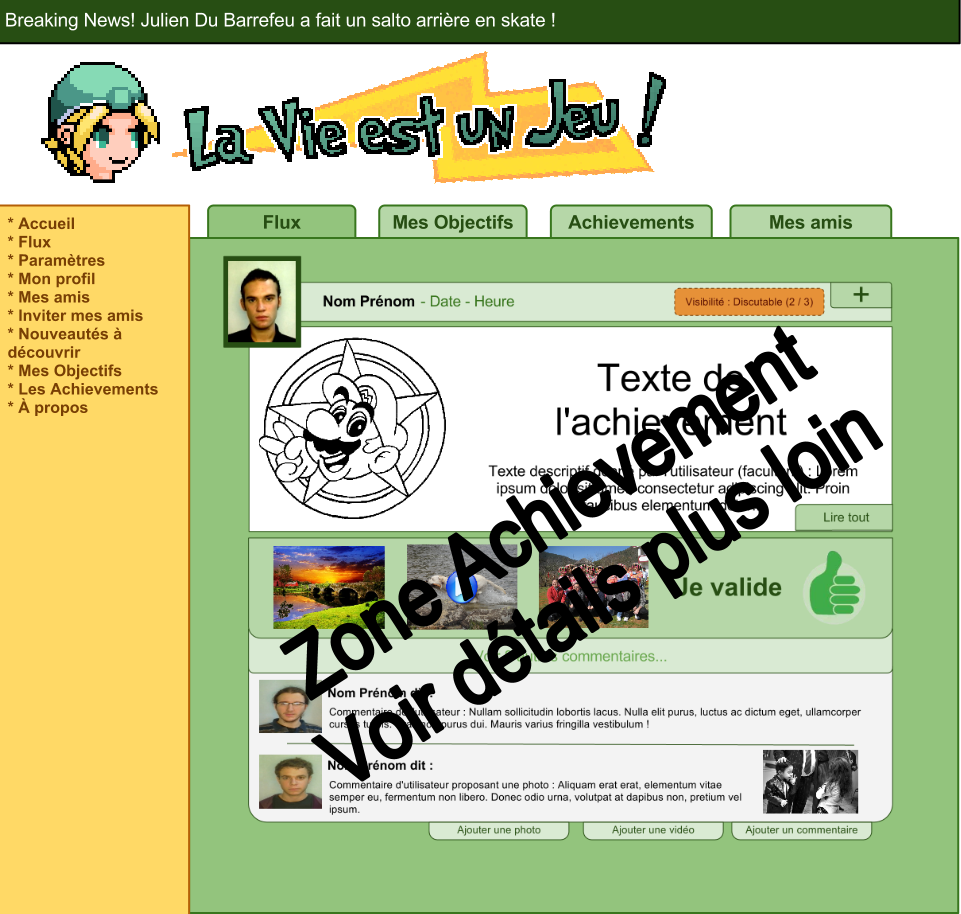
\includegraphics[width=15cm]{img/accueil.png}
  \end{center}
\end{figure}


\subsection{Onglet Flux}

L'onglet Flux sera situé au milieu de la page principale et aura pour fonction d'afficher les derniers « achievements » réalisés par le réseau social et à valider par le cercle d'amis.\\

Ce flux contiendra toutes les actions des contacts :

\begin{itemize}
  \item les « achievements » à valider (voir détails ci-dessous) ;
  \item les objectifs qu'ils se sont fixés ;
  \item les nouveaux contacts ;
  \item des nouveautés du site (informations ou nouveaux « achievements »).
\end{itemize}

\newpage

\subsection{Détails d'un « achievement »}

Chaque « achievement » disposera d'une fonction de validation à l'image des boutons ``J'aime'' de Facebook ou ``+1'' de Google+. Elle permettra aux utilisateurs d'indiquer qu'ils valident la publication en question. Le support de validation tout comme les simples commentaires pourront être au format texte, photo et/ou vidéo. La photo (ou « avatar ») de l'utilisateur apparaîtra ainsi que la description de l'« achievement », en regard de celle-ci. Il sera également possible de poster des commentaires en-dessous des preuves de validation. Un onglet « Plus » permettra de dérouler chaque « achievement » afin d'obtenir plus d'informations.\\

\begin{figure}[H]
  \begin{center}
    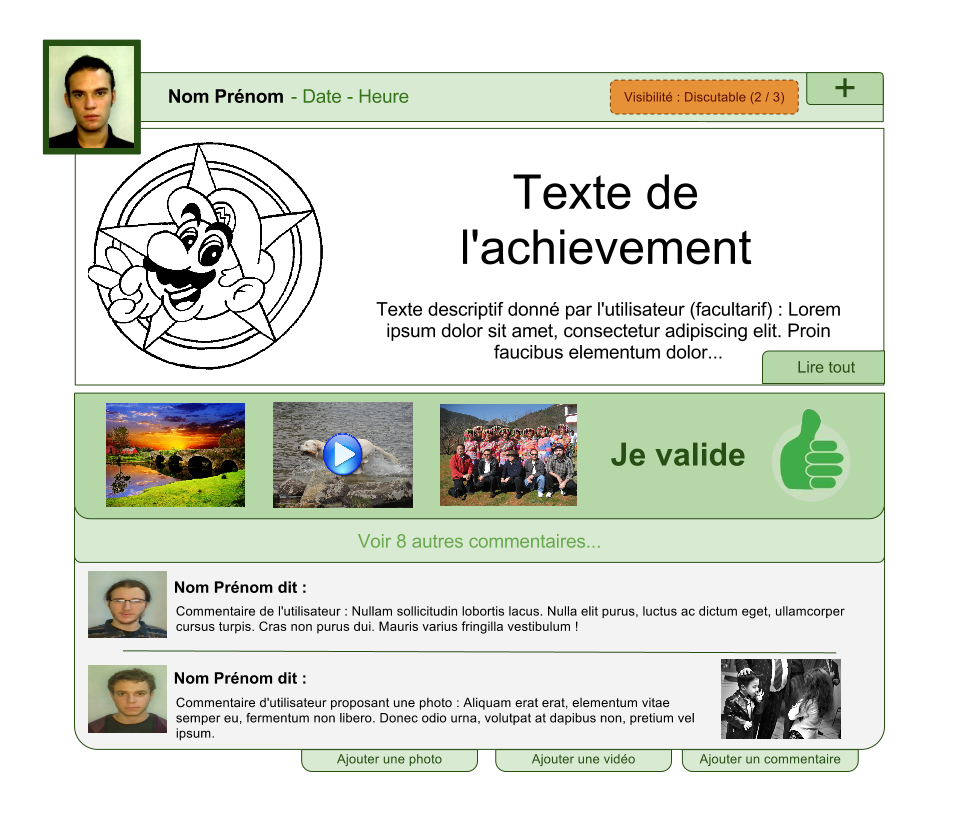
\includegraphics[width=15cm]{img/achievement.png}
  \end{center}
\end{figure}

\subsection{Onglet Achievements}

L'utilisateur pourra sélectionner des packs qui contiendront les « achievements » à accomplir. Les packs seront tous disponibles et classés par thématiques dans une sous-catégorie, mais la plateforme proposera d'abord à l'utilisateur des packs d'« achievements » correspondant aux centres d'intérêt de ce dernier, ou encore de sa tranche d'âge. Une fois un pack sélectionné, l'utilisateur peut aussi définir certains « achievements » comme étant ses objectifs, et ainsi notifier son réseau.

\subsection{Onglet Objectifs}

L'onglet Objectifs permet à l'utilisateur de construire une liste d'objectifs du quotidien ou de choses à faire absolument avant de mourir. Le but ést de filtrer les « achievements » que l'utilisateur ne désire pas réaliser dans l'immédiat et ainsi de dégager ceux qu'il va accomplir sur le court terme. La page est destinée à être régulièrement consultée : c'est à partir de cet onglet que l'utilisateur peut annoncer la fin d'un objectif, et donc obtenir un « achievement » si ses amis confirment la validation de ce dernier.

\subsection{Onglet Contacts}

L'utilisateur pourra ici voir sa liste de contacts et les profils de ceux-ci, mais aussi regrouper ses contacts par groupe. Les groupes d'utilisateurs permettent alors d'attribuer des degrés de sensibilité.\\
Le degré de sensibilité va de 0 à 3 et permet de partager les « achievements » aux contacts de son choix. Voir plus loin.

\subsection{Page Profil}

La page Profil contient les informations d'un utilisateur et permet de les modifier. Si l'utilisateur consulte la page profil d'un autre membre, il a la possibilité d'interagir avec lui de différentes manières (envoi de message, demande d'ajout dans le cercle d'amis, ...).\\
La page profil contient principalement des badges d'« achievement », tel un tableau de chasse. L'utilisateur peut cliquer sur l'« achievement » pour en avoir le détail (textes, photos, vidéos, commentaires).

\section{L'application Smartphone}

Pour ce qui est des smartphones, nous avons décidé d'utiliser des vue internet afin de développer une interface sur la base de la technologie que nous utilisons pour notre site web, à savoir Ocsigen. Cela nous permettra d'être constants dans notre ligne directrice de code. Cette interface sera chargée sur toutes les plates-formes smartphones. L'avantage de cette méthode réside dans sa totale portabilité et reste dans la continuité du défi que nous nous sommes fixés : utiliser la programmation fonctionnelle pour notre projet.

\section{L'API}

L'API permettrait d'offrir aux développeurs un accès à l'essentiel des fonctionnalités du site. On pourra y récupérer, pour un utilisateur donné, et selon les vœux de celui-ci (token d'acceptation), la liste de ses « achievements ».


%% --------------------------------------------------------------------- %%

\chapter{Une techologie nouvelle, originale et performante}

\section{Ocsigen, serveur web et puissant framework en OCaml}

La technologie utilisées s'appelle ``Ocsigen'', c'est un serveur web et un puissant framework entièrement en OCaml.\\
  \\
La programmation fonctionnelle est complètement adaptée au domaine du web comme le décrivent de nombreux articles sur internet, comme celui-ci :\\
\url{http://www-lipn.univ-paris13.fr/~loddo/funding/projet-hyper-learning.pdf}\\
\\
Son typage fort résous de nombreuses problématiques de sécurité que l'on peut rencontrer en PHP par exemple.\\

\begin{figure}[H]
  \begin{center}
    
\includegraphics[width=13cm]{img/ocsigen.png}
  \end{center}
\end{figure}

Le framework est particulièrement bien fait et propose par exemple plusieurs niveau de session : des sessions par onglets, des sessions classiques par client, des sessions par utilisateurs (connectés avec le même login à plusieurs endroits), des sessions par groupes d'utilisateurs et des sessions "persistantes" (conservées après la déconnexion).\\

\newpage

Du fait qu'il soit récent, il a  il a été pensé et conçu pour le HTML5, le Javascript et les dernières technologies côté client du web. Lorsque l'on programme avec Ocsigen, on réalise un véritable programme complet, compilé et lancé. Le language utilisé reste le même : OCaml, pour le côté client comme le côté serveur.\\
\\
OCaml facilitant la manipulation d'arbre, le code généré en HTML est fait à partir d'un AST forcément valide.\\
\\
Pour en savoir plus sur ce petit bijou :\\
\url{http://ocsigen.org/}

\section{OCaml, contraignant mais assurant stabilité et sécurité}

Les avantages et les contraites de la programmation fonctionnelle s'applique aussi dans la programmation avec Ocsigen.\\
\\
Lorsque l'on commence à écrire un programme, même s'il l'ont démarre avec de bonnes bases, on finit généralement avec une usine à gaz. Et lorsque l'on modifie quelque chose à un endroit, une autre fonctionnalité à un autre endroit qui en dépendait devient non-fonctionnelle, et il faut du temps avant que l'on s'en rende compte, bien souvent en production.\\

\begin{figure}[H]
  \begin{center}
    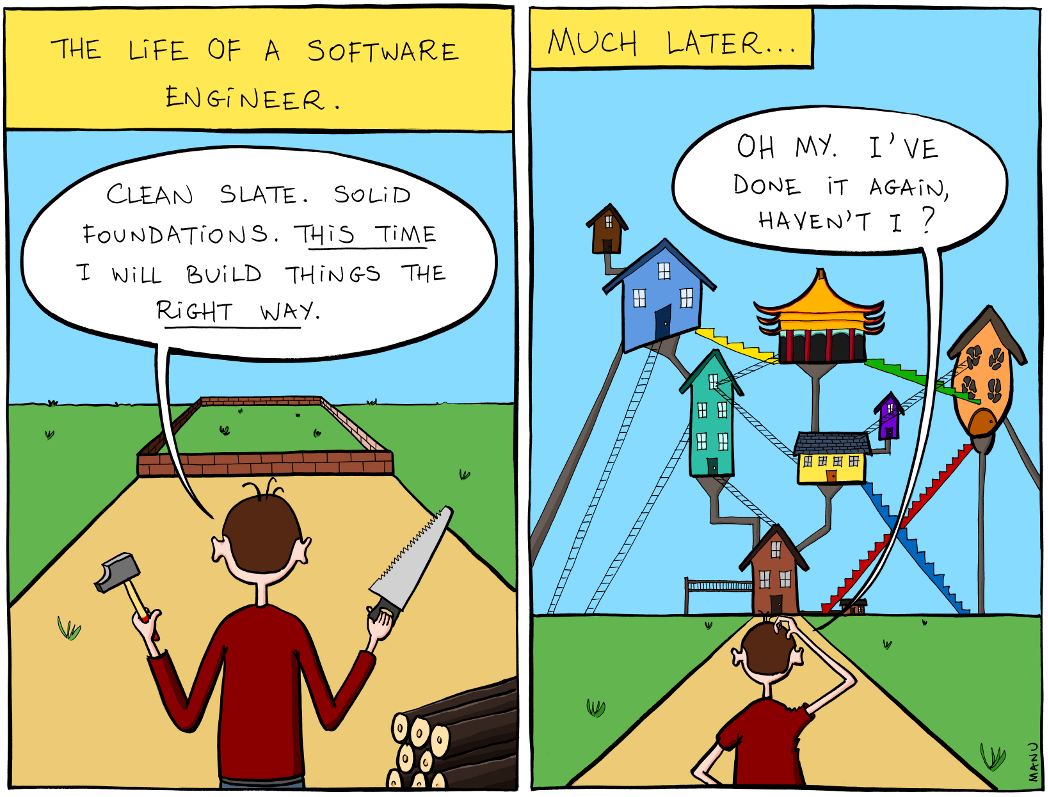
\includegraphics[width=13cm]{img/proj.png}
  \end{center}
\end{figure}

\newpage

Avec OCaml et Ocsigen, on utilise un compilateur très strict et un typage fort. Aucun écart n'est toléré !\\
Ainsi, si l'on modifie une partie du programme et que cela à un impact sur une autre fonctionnalité, alors le programme ne compilera tout simplement pas tant que tout n'est pas correct.\\

C'est très contraignant pour des développeurs qui souhaiteraient créer rapidement de petites applications sans se prendre la tête, puisqu'ils passeraient plus de temps à faire en sorte que le programme compile qu'à réaliser les fonctionnalités en elle-même.\\
Pour nous, c'est idéal. Nous savons qu'en choisissant cette technologie, nous devrons passer bien plus de temps à concevoir et réaliser notre projet que si nous avions choisi une autre technologie plus classique pour le web. Mais nos ambitions sur ce projet sont grandes et nous souhaitons nous assurer de sa sécurité, sa stabilité, ses performances, sa pureté et son absence totale de bogues. Nous savons que cette solution correspond exactement à nos attentes.
\\

\section{Portabilité client/serveur}

\subsection{Serveur}

Ocsigen est une technologie très récente. Le développement des divers services a
commencé il y a bien des années mais la mise en commun de chacun et la sortie
finale permettant de l'utiliser en production date de mars 2012 avec la sortie
de la version 2.0.\\
\\
De ce fait, le serveur Ocsigen et tout ses modules associés ne fonctionne
pour l'instant que sur très peu de distributions. Il fontionne sur certaines
distrubutions Linux connues telles que Ubuntu, Debian ou Arch Linux. À ce jour 
il ne fonctionne pas sur Microsoft Windows, Apple Mac OS X ou encore les 
distributions BSD.\\
\\
Nous avons tout de même décidé de mettre en avant l'innovation par rapport
à la portabilité sur notre projet. Notre serveur n'est donc pas portable.

\subsection{Client}

Pour palier à ce désavantage contraignant, nous avons décidé de rendre notre
service ultra portable côté client.\\
\\
Le choix de l'utilisation d'Ocsigen côté client est évidante puisque cette 
technologie est adaptée aux trois cas d'utilisation que représentent l'accès
\textit{via} un poste fixe, un smartphone ou encore une tablette. Dans le cadre
de la version web mobile Ocsigen  gère de plus de nombreuses fonctionnalités 
spécifiques aux terminaux mobiles :
\begin{itemize}
  \item Tactile (toucher simple, toucher glissé, ...)
  \item Géolocalisation
  \item Orientation
  \item Appareil photo
  \item ...
\end{itemize}

\begin{figure}[H]
  \begin{center}
    
\includegraphics[width=8cm]{img/navigateurs.png}
  \end{center}
\end{figure}

Notre service est garanti d'être utilisable sur trois types de plateformes :

\begin{itemize}
  \item Navigateurs internet classiques
    \begin{itemize}
      \item Google Chrome
      \item Mozilla Firefox
      \item Internet Explorer
      \item Apple Safari
      \item Opera
    \end{itemize}
  \item Terminaux mobiles format téléphone
    \begin{itemize}
      \item Android
      \item iOS
      \item Windows Mobile
      \item BlackBerry
    \end{itemize}
  \item Tablettes
    \begin{itemize}
      \item iPad
      \item Tablette Android
    \end{itemize}
\end{itemize}

\begin{figure}[H]
  \begin{center}
    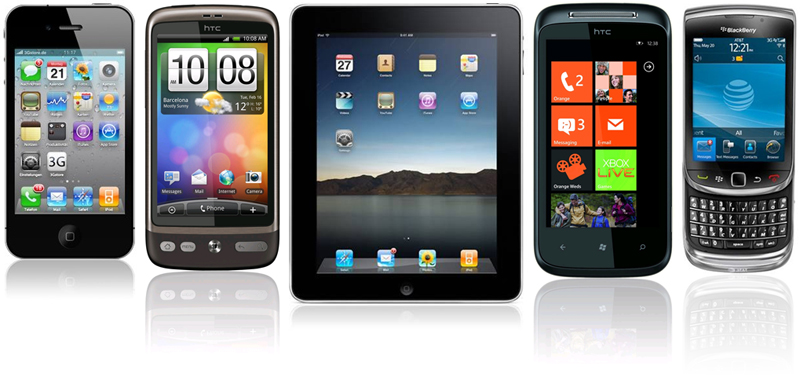
\includegraphics[width=13cm]{img/mobiles.jpg}
  \end{center}
\end{figure}

Pour chacunes de ces trois plateformes, nous aurons une interface différente
et adaptée à la résolution et aux fonctionnalités.\\
Pour chacun des types de périphériques, nous aurons un programme différent,
codé dans le langage propre à celui-ci, faisant appel à notre service Ocsigen
\textit{via} l'API développeurs détaillée par la suite.\\
En tout, nous aurons :
\begin{itemize}
  \item 3 services différents en Ocsigen
  \item 6 application mobiles différentes, dans leurs languages respectifs
\end{itemize}

On pourra donc dire que ``La Vie Est Un Jeu'' est \textbf{ultra-portable}.

%% --------------------------------------------------------------------- %%

\chapter{Description de la base de données}

\section{Description des tests de premier niveau}

\begin{itemize}
  \item Création de compte
  \item Restriction d’accès par cercles
  \item Listing des « achievements » déjà présents dans la base de données
  \item Sélection d’« achievements » parmi ceux disponibles.
  \item Pondération des « achievements ».
  \item Classement : tests des différents algorithmes de notation.
  \item Restriction des achievements pour une catégorie d’utilisateurs (ceux de niveau 3 ne seront pas accessibles au moins de 18 ans et ceux de niveau 2 aux moins de 14 ans).
\end{itemize}

\section{Schéma de la base de données}

\begin{figure}[H]
  \begin{center}
    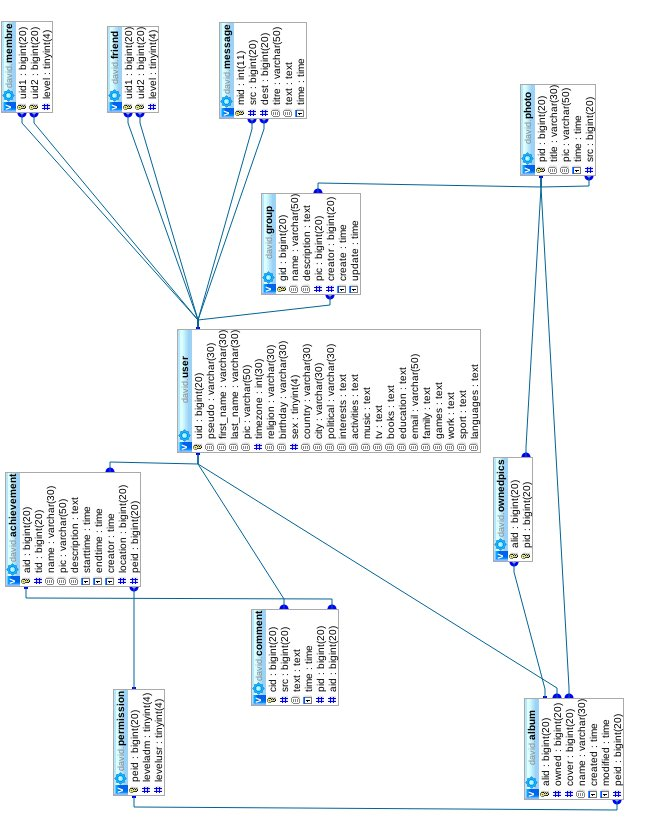
\includegraphics[width=18cm]{img/imgdb.jpg}
  \end{center}
\end{figure}

\section{Technologie et portabilité de la base de données}

Pour la base de données, nous utilisons un service qui nous ai imposé par
\textbf{Ocsigen}, la technologie que nous utilisons pour tout notre projet.\\
Ce service s'appelle \textbf{Macaque}. Il propose une approche fonctionnelle
et fortement typée de gestion de base de données.\\
Ce service est basé sur PostgreSQL et il est possible d'intéragir avec la
base de données via d'autres systèmes utilisant PostgreSQL.
Cependant, l'intéraction avec la base de données depuis notre service Ocsigen
ne peut se faire qu'avec Macaque.\\
\\
Afin de pouvoir utiliser d'autres types de bases de donnée en cas de besoin
pour la suite, nous comptons proposer des convertisseurs de base de données.\\
Nous proposerons un convertisseur PostgreSQL à MySQL dans un autre langage et
au besoin d'autres convertisseurs.

\begin{figure}[H]
  \begin{center}
    
\includegraphics[width=13cm]{img/macaque.png}
  \end{center}
\end{figure}

%% --------------------------------------------------------------------- %%

\chapter{Environnement matériel et humain de réalisation du projet}

\section{Environnement matériel}

Notre projet tourne sur un serveur Ocsigen. Il est installé sur une Dedibox PRO Dell financée par les membres du projet.

\vspace{20pt}

\begin{tabular}{|c|c|}
  \hline
   Serveur & Dell® PowerEdge R210\\
  \hline
  Processeur & 1x Intel® Xeon® L3426\\
  \hline
  Architecture & 4x 1.86GHz, 64 Bits, Virtualisation\\
  \hline
  Mémoire vive & 16 Go DDR3 ECC\\
  \hline
  Disque dur & 2 x 2 To SATA2 Raid 0 / Raid 1 HARD (H200)\\
  \hline
  Prix mensuel & 49,99 euros HT\\
  \hline
\end{tabular}

\vspace{20pt}

\section{Coûts}

\begin{itemize}
  \item Un compte développeur pour chaque boutique d'application (iOS : AppStore (99\$), Google Play (Android : 25\$) et Marketplace Windows Phone (99\$)) pour les applications mobiles.
  \item Un serveur dédié, dans un premier temps taillé pour le développement du site pouvant gérer seulement peu d'utilisateurs connectés en même temps à environ 60 euros par mois.
  \item Un serveur de production, qui sera utilisé ultérieurement pouvant aller jusqu'à 600 euros par mois.
  \item Nous envisageons par la suite, une fois l'application complétement terminée, d'engager un graphiste pour les « achievements ».
\end{itemize}

\section{Environnement et outils de réalisation}

Afin de communiquer et d’échanger sur le projet, notre groupe de travail s’appuie sur plusieurs outils.

\begin{itemize}
  \item Le projet dispose de son canal IRC officiel (\#life-eip sur irc.epitech.net), dont le but est d’assurer un support rapide aux utilisateurs et contributeurs en gérant une historique des discussions.
  \item Additionnellement, l’équipe du projet a accès à une mailing list (hébergée par google groups).
  \item Elle gère tous les documents relatifs à l’évolution du projet grâce aux google documents.
  \item La documentation se trouve sur le site vitrine : \url{http://eip.epitech.eu/2014/lavieestunjeu/}
  \item Nous avons un bug tracker, un wiki et des tickets sur un dépôt privé GitHub.
\end{itemize}

\section{Architecture technique}

\begin{itemize}
  \item Le projet se base sur un environnement Web en OCaml, donc la composante principale est le serveur web \href{http://ocsigen.org/}{Ocsigen}.
  \item Le projet s’appuiera également sur \href{http://ocsigen.org/js_of_ocaml/}{js\_of\_ocaml}, un outil de compilation d’OCaml en JavaScript.
  \item Il gèrera une base de données grâce à \href{http://ocsigen.org/macaque/}{Macaque}, un autre projet initié par l’INRIA.
\end{itemize}

Pour plus de détails, reportez-vous au chapitre sur les technologies utilisées.

\section{Sécurité des informations utilisateurs}

\begin{itemize}
  \item Mise en place d’une solution de « niveau de confidentialité », un utilisateur pourra définir un niveau de confidentialité pour chaque utilisateur de son réseau. 

\begin{figure}[H]
  \begin{center}
    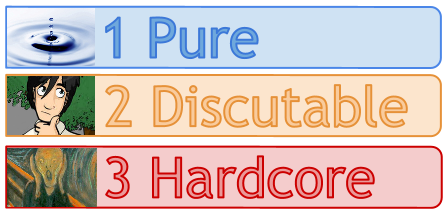
\includegraphics[width=10cm]{img/confidentialite.png}
  \end{center}
\end{figure}

\end{itemize}

\section{Points sensibles}

\begin{itemize}
  \item La sécurité des informations est une priorité pour nous. Nous ferons donc très attention à ce que les utilisateurs sachent toujours à tout moment qui a accès à quelles informations.
  \item Nous souhaitons conserver notre idée secrète jusqu’à ce que nous ayons une version de base utilisable.
  \item La stabilité et la sécurité est notre priorité et sera assuré grâce à l'utilisation d'Ocsigen.
\end{itemize}

%% --------------------------------------------------------------------- %%

\chapter{Organisation projet}

\section{Planning}

D'un point de vue global, le projet se déroulera en trois grandes parties : documentation, développement et mise en production.\\

\subsection{ Première année : Documentation, Conception}

Avant de passer à la réalisation concrète du produit, nous allons nous consacrer à la rédaction de plusieurs documents essentiels au bon déroulement du projet. En effet, il est nécessaire de définir précisément les détails du projet, la conception, étudier les différents outils et technologies à notre disposition et faire des choix, ou encore mettre en place des partenariats.\\
Parmi les documents réalisés, on trouve :

\begin{itemize}
  \item 50 mots
  \item Étude de l'existant
  \item Étude détaillée
  \item Cahier des Charges (3 versions)
  \item Diagramme de Gantt
  \item Bilan Architecture
\end{itemize}

Nous continuerons cette étude jusqu'en septembre 2012.\\

\newpage

\subsection{ Deuxième année : Développement, Code, Tests}
Une fois les outils en main, les spécificités définies et les rôles attribués, nous commencerons à développer le produit.\\
\begin{itemize}
  \item Hello World! (01/08/12)
  \item \textbf{Login} : (01/08/12)
  \item Formulaire site web (01/08/12)
  \item Facebook/Google+ (01/08/12)
  \item Page d'accueil (01/08/12)
  \item \textbf{Gestion BDD} : (01/08/12)
  \item Déploiement BDD (01/08/12)
  \item Catégories et sous-catégories d'achievements (29/08/12)
  \item Parcours de catégories (29/08/12)
  \item Achievements simples (29/08/12)
  \item Gestion des contacts (01/10/12)
  \item Contacts Facebook/Google+ (01/10/12)
  \item Mise en place sécurité et partage (01/10/12)
  \item Partage Facebook/Google+ (01/11/12)
  \item Création de Flux (01/11/12)
  \item \textbf{Gestion achievements} : (01/11/12)
  \item Texte personnalisé (01/12/12)
  \item Vidéos et photos (01/11/12)
  \item Commentaires simples (01/01/13)
  \item Commentaires vidéos et photos (01/01/13)
  \item Page de profil utilisateurs (01/01/13)
  \item Objectifs d'achievements par utilisateurs (01/02/13)
  \item Filtrage pour affichage de flux (01/01/13)
  \item Finalisation utilisateurs (avatars, infos...) (01/02/13)
  \item Finalisation achievements (01/03/13)
  \item Guide découverte site (01/04/13)
  \item Finalisation du site / Phase de tests (01/04/13)
  \item Sortie d'une première version du site (01/06/13)
\end{itemize}

En fin de deuxième année, après la finalisation du projet, nous consacrerons au minimum un mois à des tests avant la mise en production. Ces tests seraient \\
Nous pensons mettre en production une version finale pour septembre 2013.\\

\subsection{ Troisième année : Mise en production, partennariats commerciaux, création d'entreprise}

La dernière période sera consacrée aux problématiques de communication, et dans une moindre mesure de développement. Ainsi, durant la dernière année du projet, nous tâcherons de faire connaître ce dernier de diverses façons, pour créer la communauté indispensable à notre plateforme, en plus de la finalisation technique du produit. Nous pourrons de ce fait bénéficier de retours d'utilisateurs, afin de corriger les anomalies et peaufiner la plateforme.\\
Nous souhaitons obtenir des partennariats commerciaux pour faire connaître notre plateforme.\\
Nous souhaitons inscrire notre projet à de nombreux concours d'innovations et de jeunes entreprises afin d'obtenir une visibilité et un public et pourquoi pas des financements supplémentaires.\\
\\
En un mot, la troisième année sera consacrée à faire de ce projet un \textbf{succès}.

\begin{figure}[H]
  \begin{center}
    
\includegraphics[width=12cm]{img/corporate.jpg}
  \end{center}
\end{figure}

\newpage

\section{L'Équipe}

Durant la période de développement du produit, l'équipe sera dispersée dans plusieurs pays, rendant tout travail en équipe difficile. Nous allons nous répartir les tâches de manière à pouvoir travailler de façon relativement autonome : notre projet étant composé de plusieurs éléments distincts, nous nous arrangerons pour ne pas en partager un entre des membres situés dans des lieux différents.\\

\subsection{ Répartition des rôles}

Ci-dessous la liste des responsables assignés à chaque catégories de tâches à
réaliser.\\
Les responsables ne sont pas forcément ceux qui réaliseront les tâches, mais ce
seront eux qui auront pour responsabilité de faire en sorte que celles-ci soient
réalisés, en les faisant eux-même ou en répartissant le travail.

\subsection{ Documentation, conception}

\begin{itemize}
  \item \textbf{Guillaume Caradec} s'occupe de la gestion générale de projet
  \item \textbf{Barbara Lepage} dirige la partie technique.
  \item \textbf{Barbara Lepage} est responsable site vitrine
  \item \textbf{Barbara Lepage} est responsable documentation
  \item \textbf{David Lassagne} est responsable conception
  \item \textbf{Barbara Lepage} est responsable formation OCaml et Ocsigen
  \item \textbf{Nicolas Klarman} est grand maître des « achievements »
\end{itemize}

\subsection{ Développement, code, tests}

\begin{itemize}
  \item \textbf{Barbara Lepage} est responsable développement des applications côté
    serveur
  \item \textbf{Guillaume Louvigny} est responsable développement des
    applications côté client pour l'interface web
  \item \textbf{Guillaume Caradec} s'occupe de l'érgonomie, des interfaces, du
    design général
  \item \textbf{David Lassagne} est responsable architecture base de données
  \item \textbf{Guillaume Louvigny} est responsable SQL
  \item \textbf{Wilfried Le-Cor} est responsable développement Android
  \item \textbf{François Glorieux} est responsable développement Windows
  \item \textbf{Youssef El-Outmani} est responsable développement Blackberry
  \item \textbf{Nicolas Klarman} est responsable développement iOS
  \item \textbf{Frank Lenormand} est responsable multimédia (photos, vidéos, ...)
  \item \textbf{Guillaume Louvigny} est responsable réseaux sociaux (Facebook,
    Google+, Twitter, ...)
  \item \textbf{Frank Lenormand} est responsable commit
  \item \textbf{Simon Corsin} est responsable développeurs tiers (API)
  \item \textbf{Wilfried Le-Cor} est responsable intéraction utilisateurs
  \item \textbf{Nicolas Klarman} est responsable Gameplay
  \item \textbf{François Glorieux} est responsable aspect communautaire
  \item \textbf{Simon Corsin} est responsable des tests de mise en production
\end{itemize}

\subsection{ Communication, entreprise}

\begin{itemize}
  \item \textbf{Guillaume Caradec} est responsable communication
  \item \textbf{Guillaume Caradec} est responsable commercial
  \item \textbf{Barbara Lepage} est responsable entreprise
  \item \textbf{Barbara Lepage} est responsable innovation
  \item \textbf{Barbara Lepage} est responsable financement
\end{itemize}

\subsection{ Outils}

Nous avons à notre disposition divers outils pour nous organiser et communiquer plus facilement :\\

\begin{itemize}
  \item une mailing-list et un canal IRC, permettant de traiter l'ensemble des diverses problématiques ;
  \item un dossier Google Docs, pour pouvoir partager les documents liés au projet et leur rédaction ;
  \item Gtalk, une application de Google permettant d'organiser des visio-conférences via un navigateur ;
  \item un dépôt Git ;
  \item l'utilisation de Doodle, pour planifier plus facilement les réunions.
\end{itemize}

Les membres du groupe se réuniront \textbf{toutes les semaines} pour parler de l'avancement du projet, des imprévus rencontrés et des objectifs à court terme.


\section{Planning détaillé avec dates précises}

Veuillez vous reporter au fichier joint \texttt{2014\_GAN3\_FR\_lavieestunjeu.pdf}. Il contient le diagramme de Gantt de notre projet.

%% --------------------------------------------------------------------- %%

\chapter{Conclusion}

\section{Conclusion du document}

Ce document présentait donc les spécification de notre EIP, La Vie est un Jeu.\\
\\
Nous y avons décrit l'ensemble des fonctionnalités qui seront proposées, ce qui inclue à la fois le site web ainsi que les applications mobiles.\\
\\
Était également présenté la définition de la base de données applicable sur toutes les plates-formes visées.\\
\\
L’API à destination de développeurs tiers avait également été définie.\\
\\
Pour finir, il détaillait également ceux à qui se destine le projet, et estimait les diverses contraintes imposées par celui-ci qu’elles soient d’ordre financières ou organisationnelles.\\

\section{SWOT}

\begin{figure}[H]
  \begin{center}
    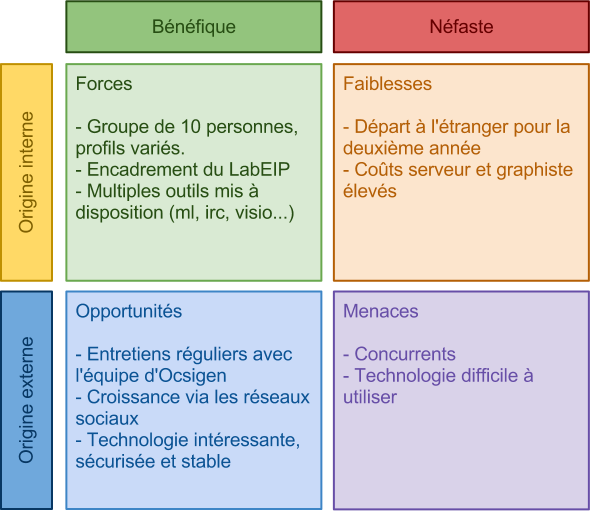
\includegraphics[width=14cm]{img/swot_fr.png}
  \end{center}
\end{figure}

%% --------------------------------------------------------------------- %%

\chapter{Annexes}

\section{Localisation des membres de l'équipe durant la deuxième année de réalisation du projet}

\begin{tabular}{|c|c|}
  \hline
  Lepage Barbara & Long Beach et Berkey, États-Unis\\
  \hline
  Caradec Guillaume & Paris, France\\
  \hline
  Corsin Simon & Paris, France\\
  \hline
  Glorieux François & Université de Beijing, Chine\\
  \hline
  Klarman Nicolas & Paris, France\\
  \hline
  Lassagne David & Université de Beijing, Chine\\
  \hline
  Louvigny Guillaume & Paris, France\\
  \hline
  El-Outmani Youssef & Université de Beijing, Chine\\
  \hline
  Le-Cor Wilfried & Suède\\
  \hline
  Lenormand Frank & Finlande\\
  \hline
\end{tabular}

\newpage

\section{Glossaire}


\begin{description}
\item[Algorithme]
Suite finie et non-ambiguë d’instructions permettant de donner la réponse à un problème.
\item[API]
En français ``interface de Programmation'', est une interface fournie par un programme informatique permettant l'interaction des programmes les uns avec les autres.

\item[Application mobile]
Une application mobile est une application développée pour être installée sur un appareil électronique mobile.

\item[Architecture Web]
Architecture Web désigne la structure générale inhérente à un environnement web.

\item[Base de données]
Une base de données est un lot d'informations stockées dans un dispositif informatique.

\item[Breaking news]
En français ``Dernières Nouvelles''.

\item[Bug tracker]
En français ``Logiciel de suivi de problèmes'',  logiciel permettant d'aider les utilisateurs et les développeurs à améliorer la qualité d'un logiciel en trouvant les failles dudit logiciel.

\item[Cahier des charges]
Le Cahier des charges vise à définir simplement les spécifications d’un produit ou d’un service à réaliser.

\item[Dépôt]
Un dépôt est un stockage centralisé et organisé de données.

\item[Diagramme de Gantt]
Un diagramme de Gantt est un outil utilisé en ordonnancement et gestion de projet et permettant de visualiser dans le temps les diverses tâches liées composant un projet.

\item[Diaporama]
Un diaporama est une suite d’images ou de documents reliés par des effets et sur lesquels il est possible de mettre du son.

\item[Doodle]
Doodle.com est un site web de planification et de sondage de la société suisse Doodle AG.

\item[GitHub]
Github est un service Web d'hébergement et de gestion de développement de logiciels, utilisant le programme Git. 

\item[Google Docs]
Google Docs est la suite des évolutions de Google Spreadsheets, logiciel de traitement de texte. Ces programmes fusionnés permettent un travail collaboratif en ligne.

\item[Google Talk]
Google Talk est un logiciel propriétaire et service de messagerie instantanée et de voix sur IP basé sur Jabber et développé par la société Google.

\item[IRC]
IRC est un protocole de communication textuelle sur internet.

\item[JavaScript]
JavaScript est un langage de programmation de scripts principalement utilisé pour les pages Web interactives.

\item[Login]
En français ``Identifiant'', information permettant à une personne de s'identifier auprès d'un système.

\item[Mailing list]
En français ``Liste de diffusion'', utilisation spécifique du courrier électronique qui permet le publipostage d'informations aux utilisateurs qui y sont inscrits.

\item[Mise en production]
Mise à disposition ``totale'' d’un service ou d’un produit.

\item[Ocaml]
Anciennement connu sous le nom d'Objective Caml, c’est l'implémentation la plus avancée du langage de programmation Caml.

\item[Ocsigen]
Framework de développement Web, développé par le laboratoire français PPS.

\item[Réseau]
Maillage de liens entre différents équipements informatiques permettant un partage d’informations.

\item[Réseau social]
Ensemble d'identités sociales, telles que des individus ou encore des organisations, reliées entre elles par des liens créés lors d’interactions sociales.

\item[Service]
Apporte une valeur ajoutée à un produit ou assure un travail nécessaire à une entreprise ou à un particulier.

\item[Site vitrine]
Site internet composé de quelques pages présentant une société. Permet à une entreprise de communiquer avec le monde.

\item[Smartphone]
Téléphone mobile disposant aussi des fonctions d'un assistant numérique personnel. Il fournit des fonctionnalités basiques comme l'agenda, le calendrier, la navigation sur le web, la consultation du courrier électronique, de messageries instantanées, le GPS...

\item[Android]
Système d’exploitation utilisant le noyau Linux pour smartphones, PDAet terminaux mobiles conçu par Android, une startup rachetée par Google.

\item[iOS]
Système d’exploitation mobile développé par Apple pour l'iPhone, l'iPod touch, et l'iPad. Il est dérivé de Max OS X dont il partage les fondations.

\item[Windows Phone]
Système d’exploitation mobile développé par Microsoft pour succéder à Windows Mobile, sa précédente plateforme logicielle.

\item[Version Bêta]
Version de test comportant toutes les fonctionnalités d'un programme. C'est grâce à cette version que les testeurs remontent les éventuels problèmes.

\item[Wiki]
Espace collaboratif sur lequel les utilisateurs sont invités à rédiger des documents de travail.


\end{description}
\end{document}
